\appendix
\chapter{Simulation Graphs}

\begin{figure}
    \centering
    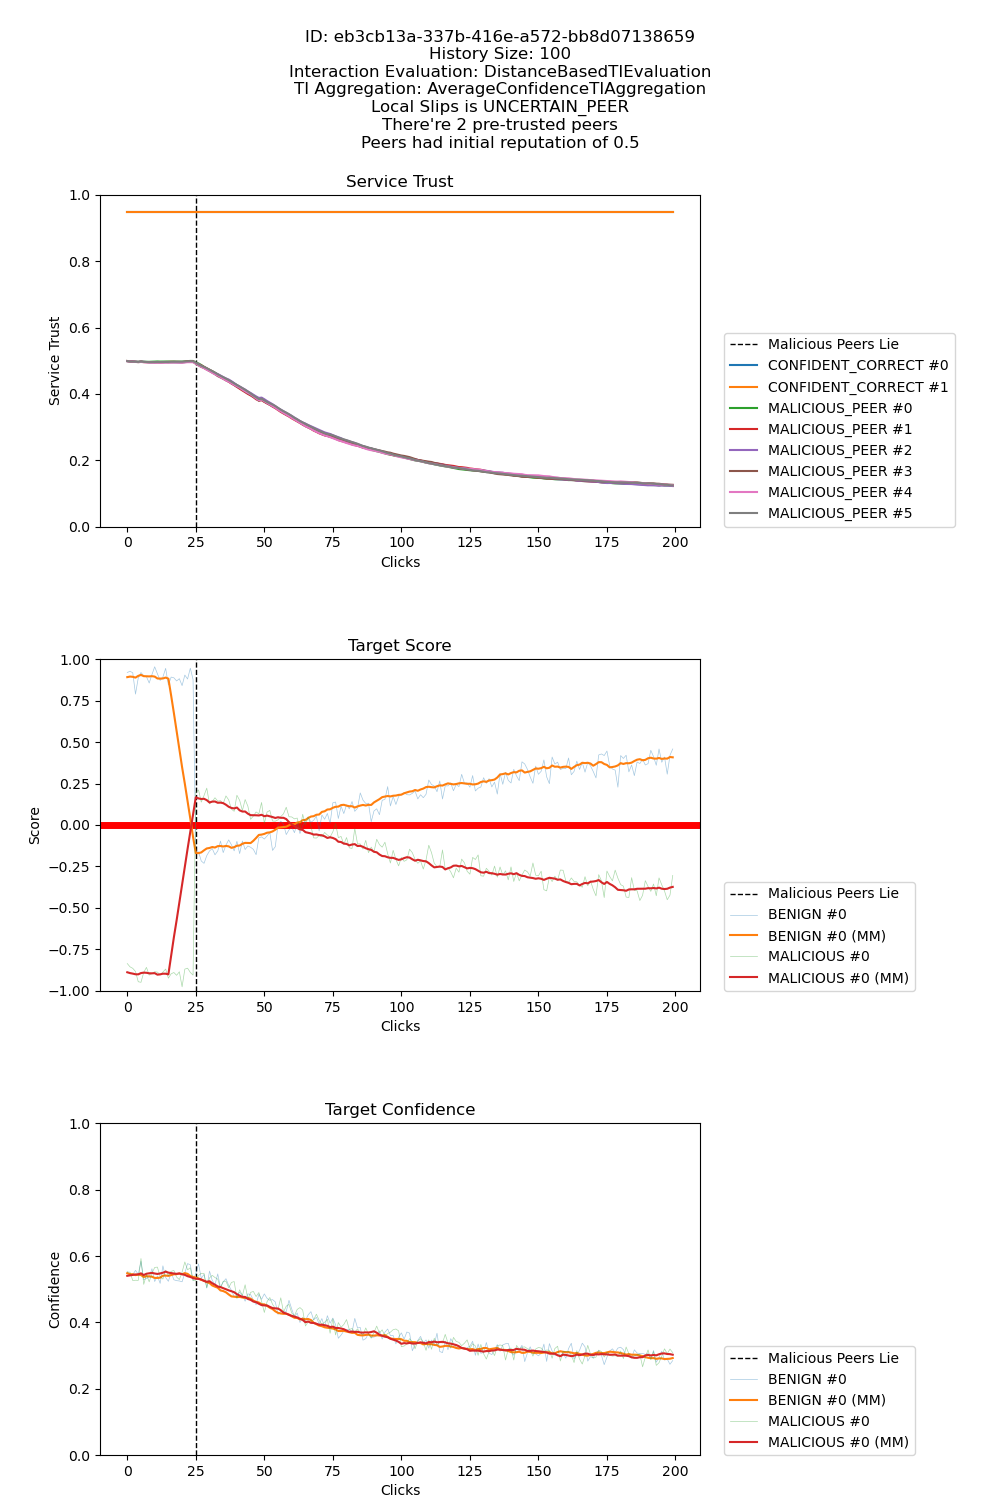
\includegraphics[width=0.95\textwidth]{assets/miss_classification_recovery.png}
    \caption{A scenario when the malicious peers overcame Fides after they started lying but only for a short period of time. Once Fides realize that the peers are lying, it lowered their service trust and the it was able to recover the score to the correct values.}
    \label{fig:missclassification-recovery}
\end{figure}

\begin{figure}
    \centering
    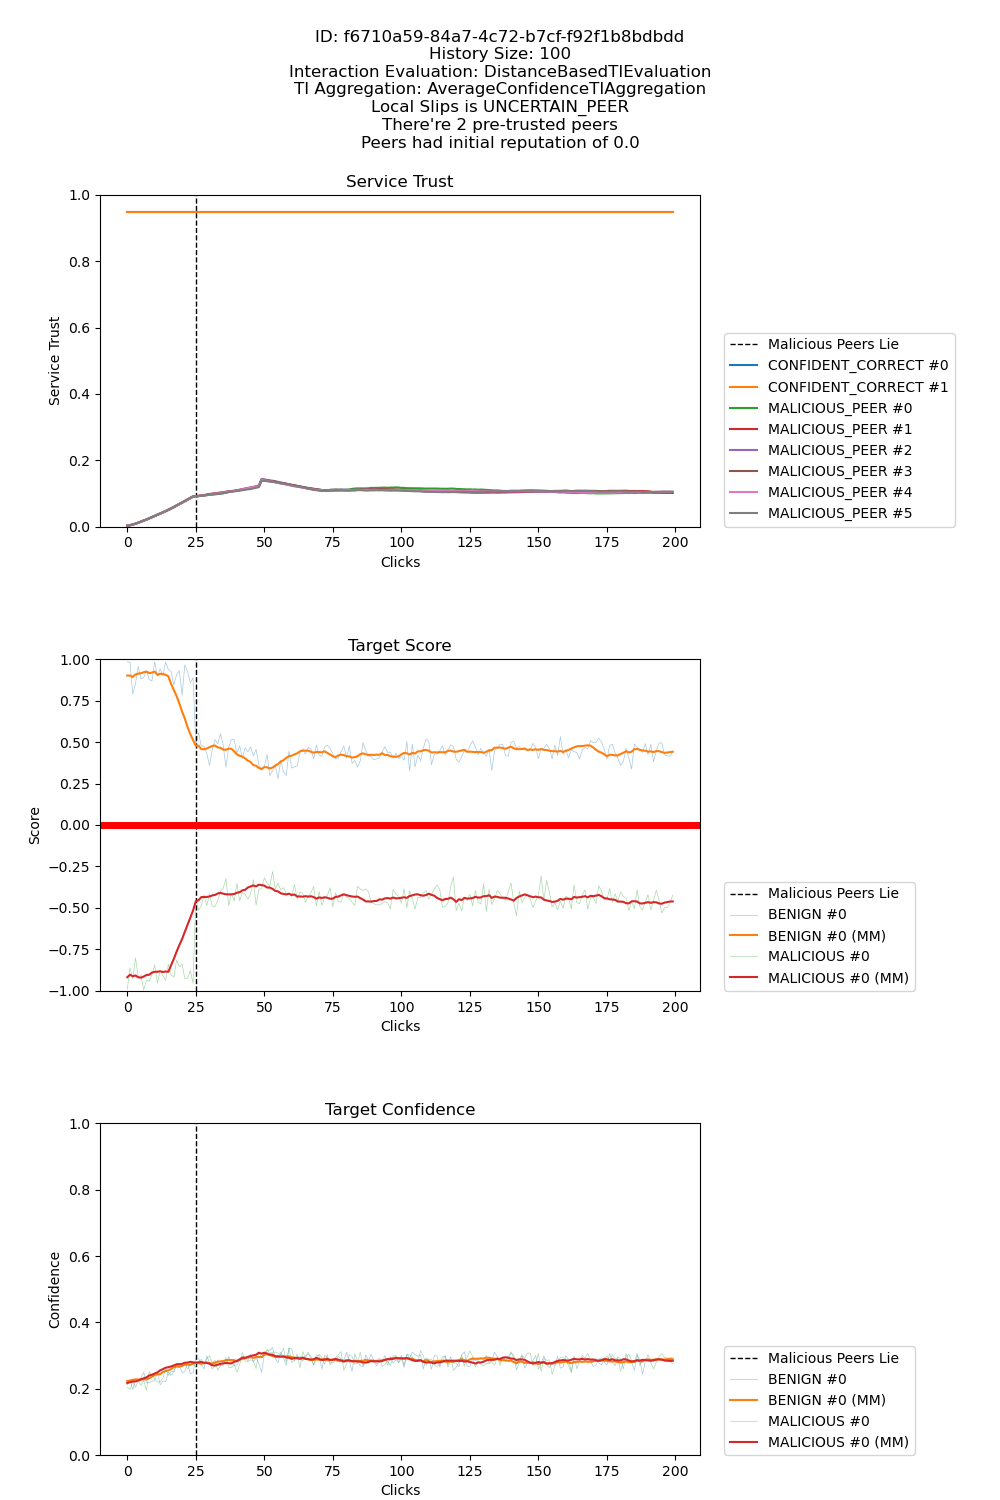
\includegraphics[width=0.95\textwidth]{assets/best_worst_case}
    \caption{The scenario where there are 75\% of the peers malicious and l}
    \label{fig:worst-best-scenario}
\end{figure}

\begin{figure}
    \centering
    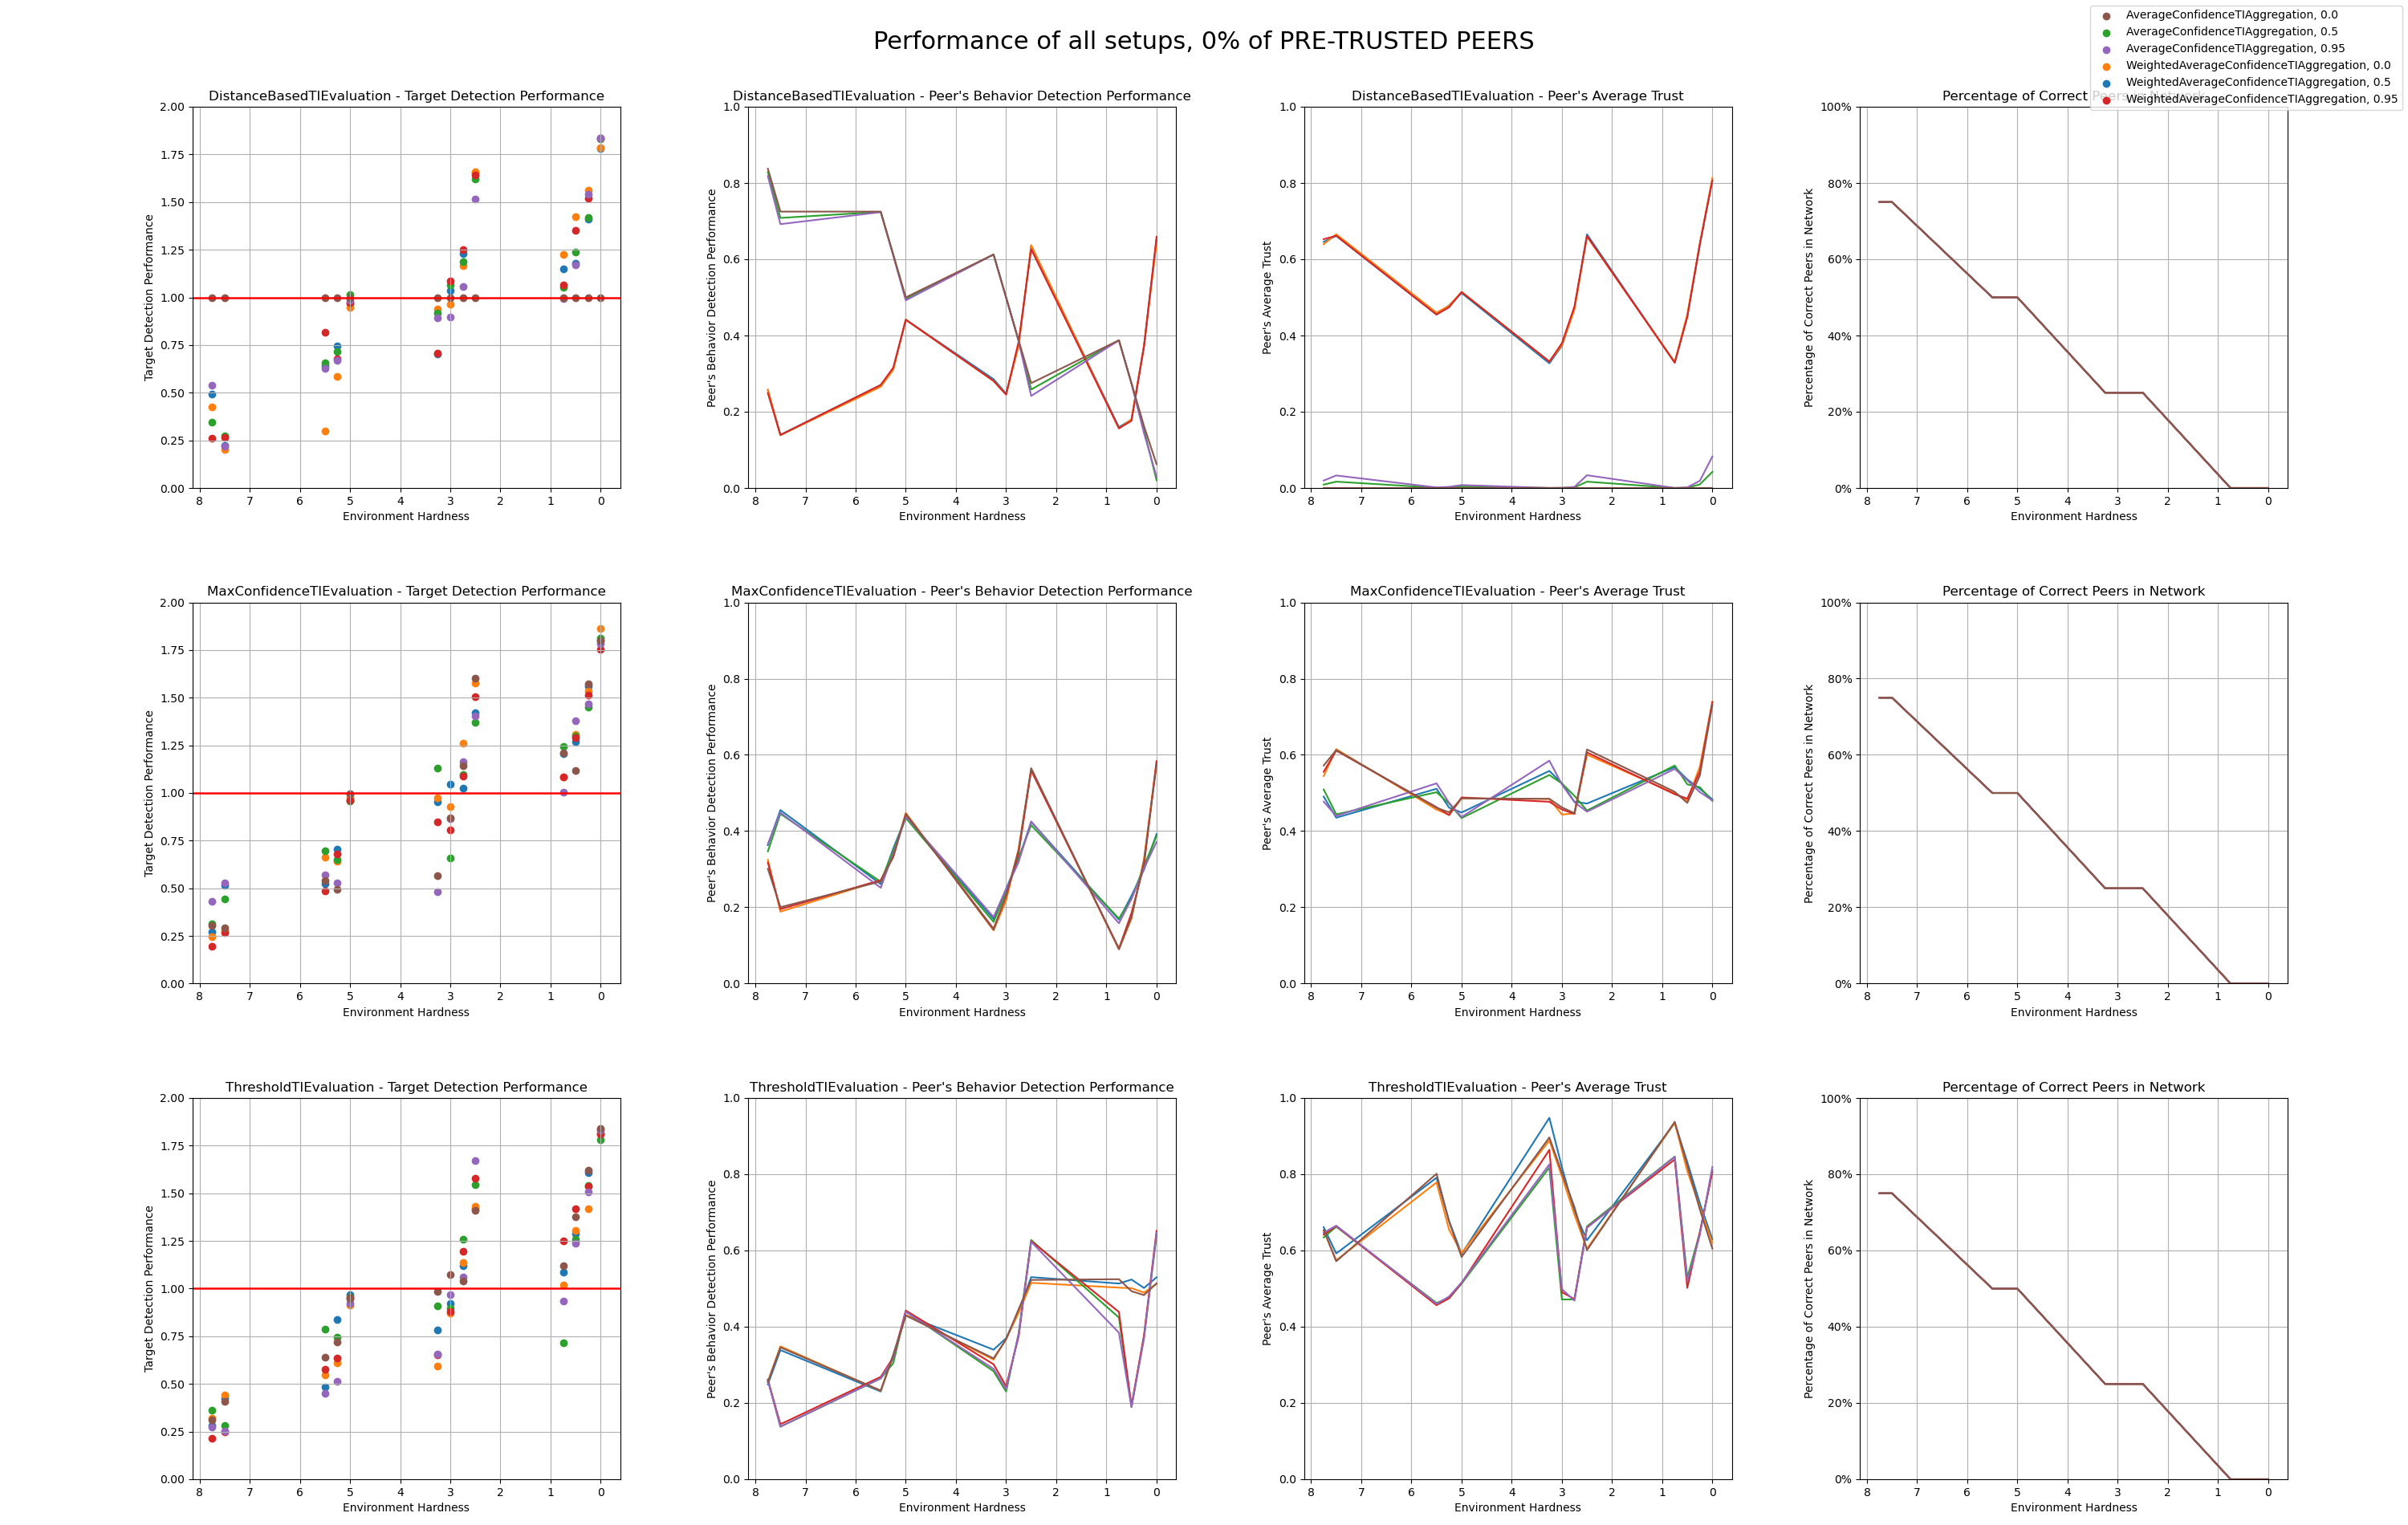
\includegraphics[width=0.9\paperwidth, angle=90]{assets/0_all_metrics.png}
    \caption{Evaluation of performance of all trust model setups with no pre-trusted peers}
    \label{fig:performance-all-setups-0-pretrusted}
\end{figure}

\begin{figure}
    \centering
    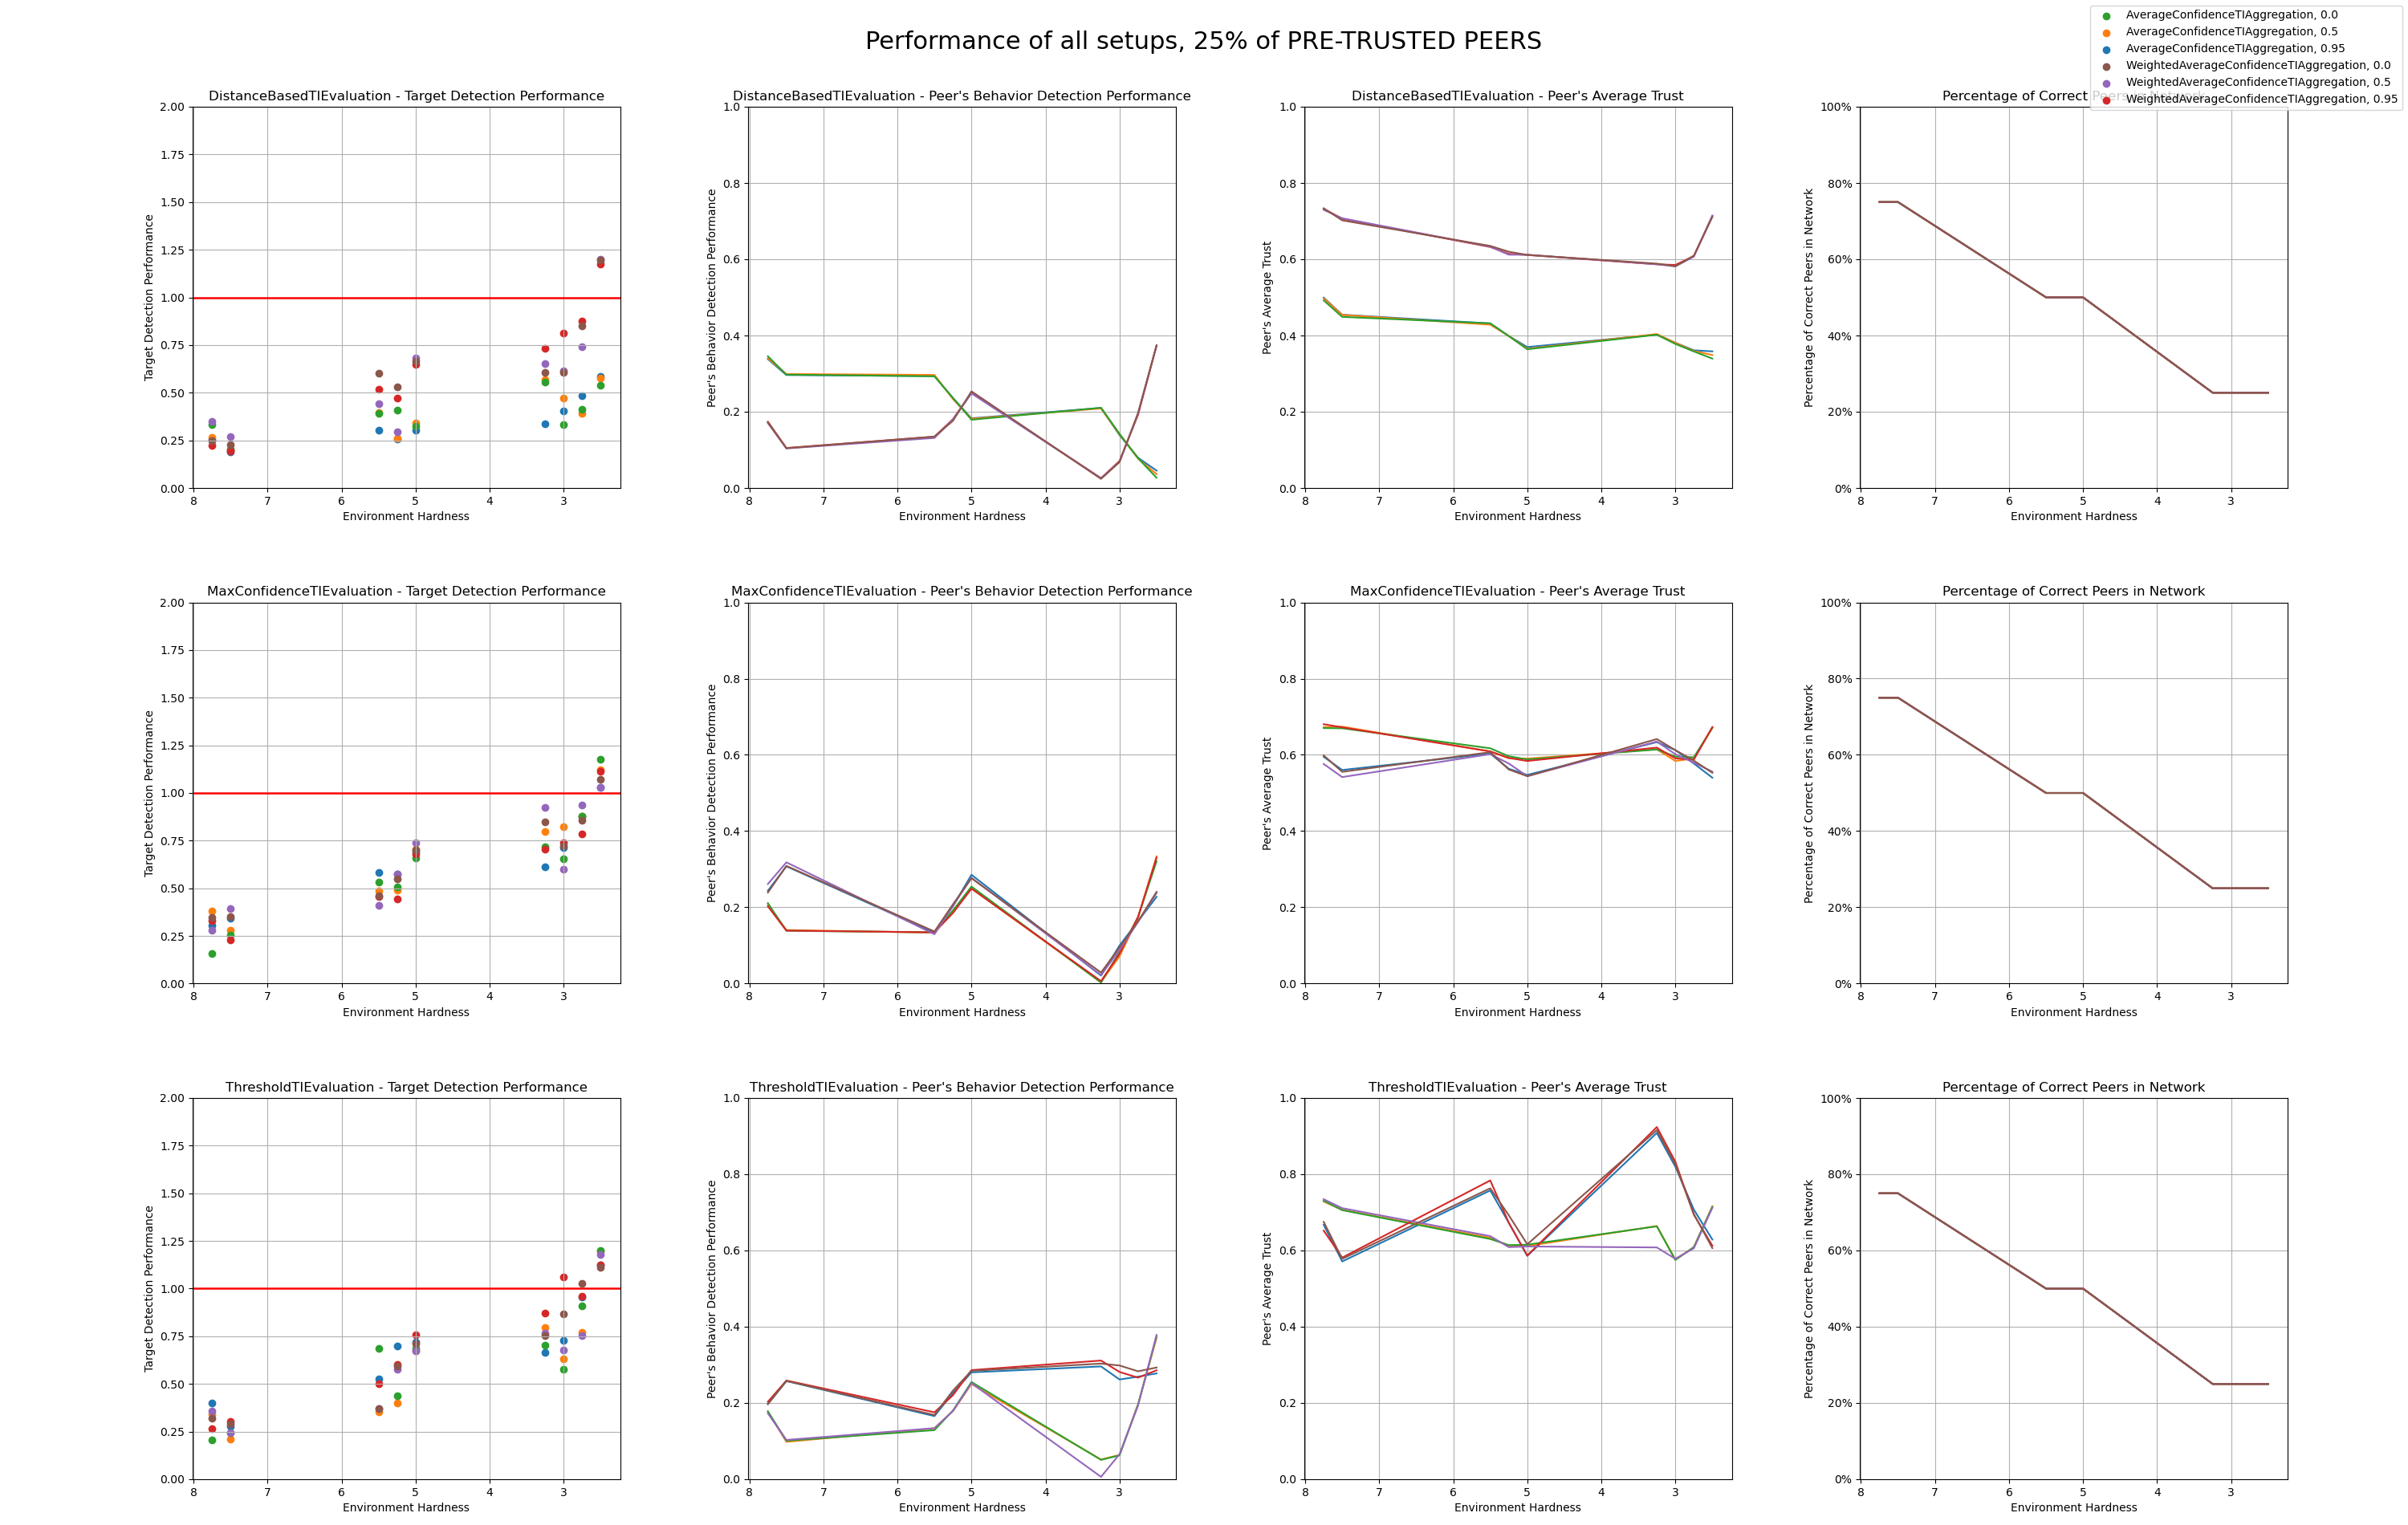
\includegraphics[width=0.9\paperwidth, angle=90]{assets/25_all_metrics.png}
    \caption{Performance of all setups with 25\% pre-trusted peers}
    \label{fig:performance-all-setups-25-pretrusted}
\end{figure}

\begin{figure}
    \centering
    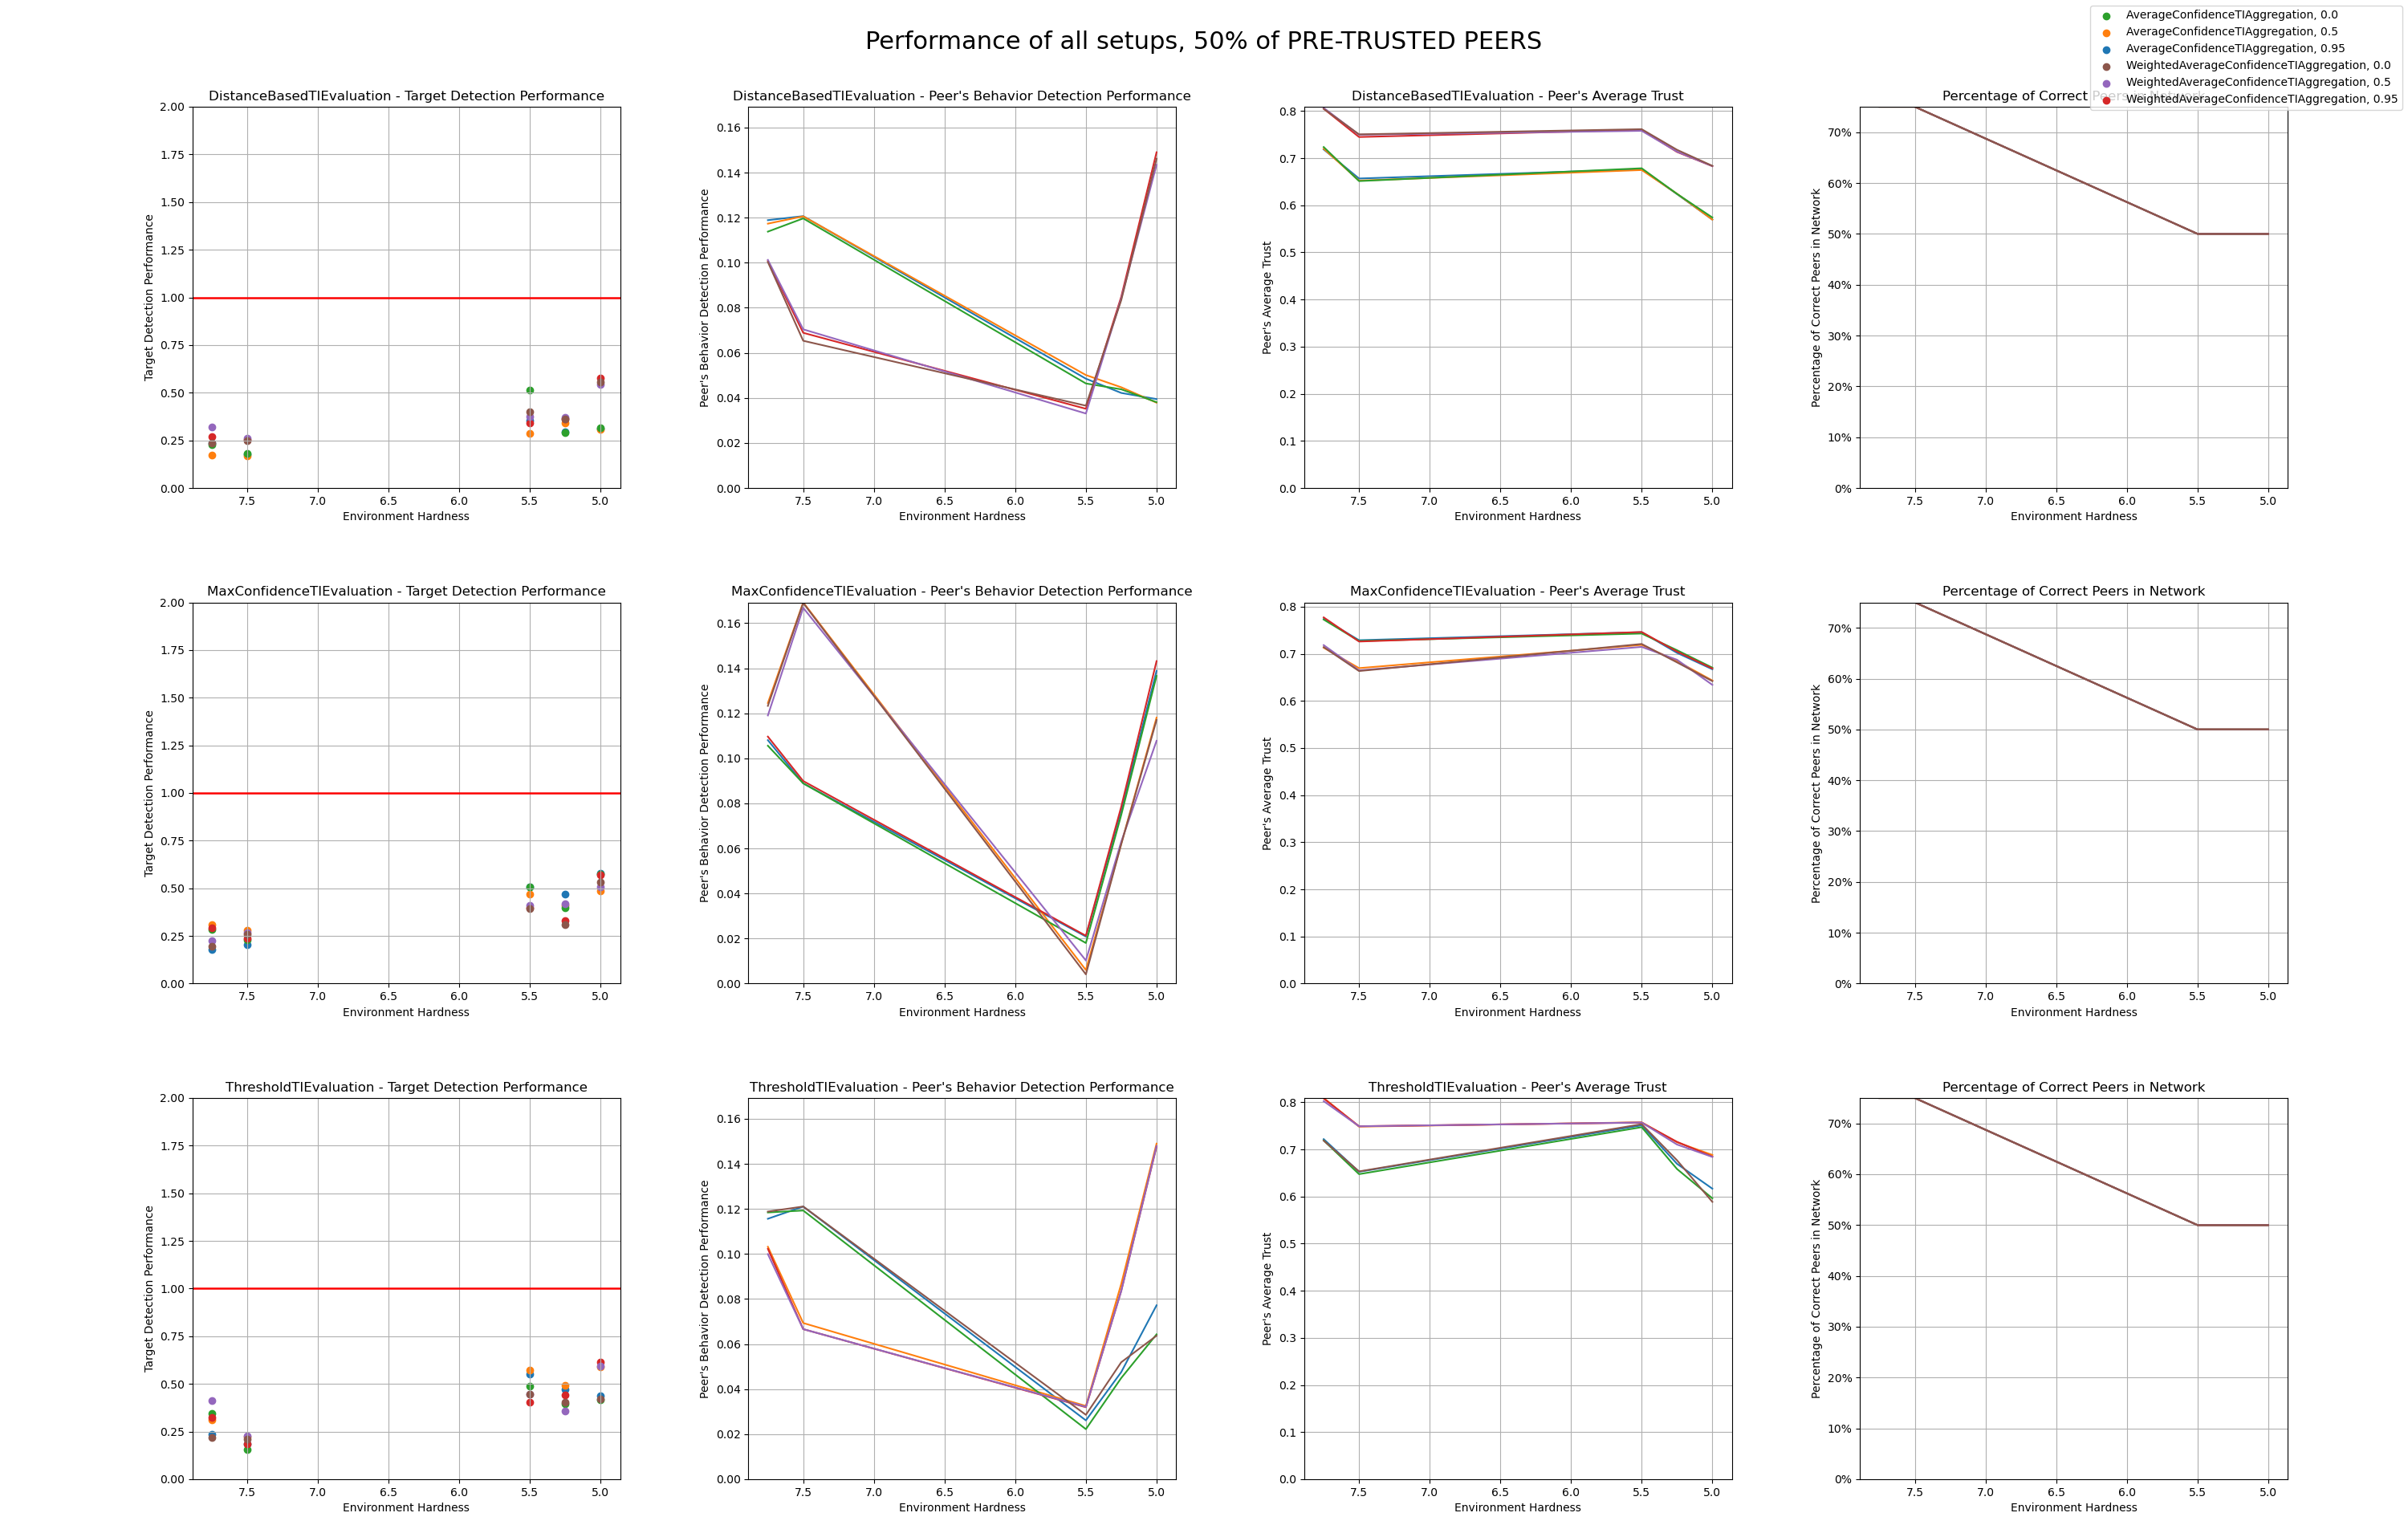
\includegraphics[width=0.9\paperwidth, angle=90]{assets/50_all_metrics.png}
    \caption{Evaluation of performance of all trust model setups with 50\% of pre-trusted peers}
    \label{fig:performance-all-setups-50-pretrusted}
\end{figure}

\begin{figure}
    \centering
    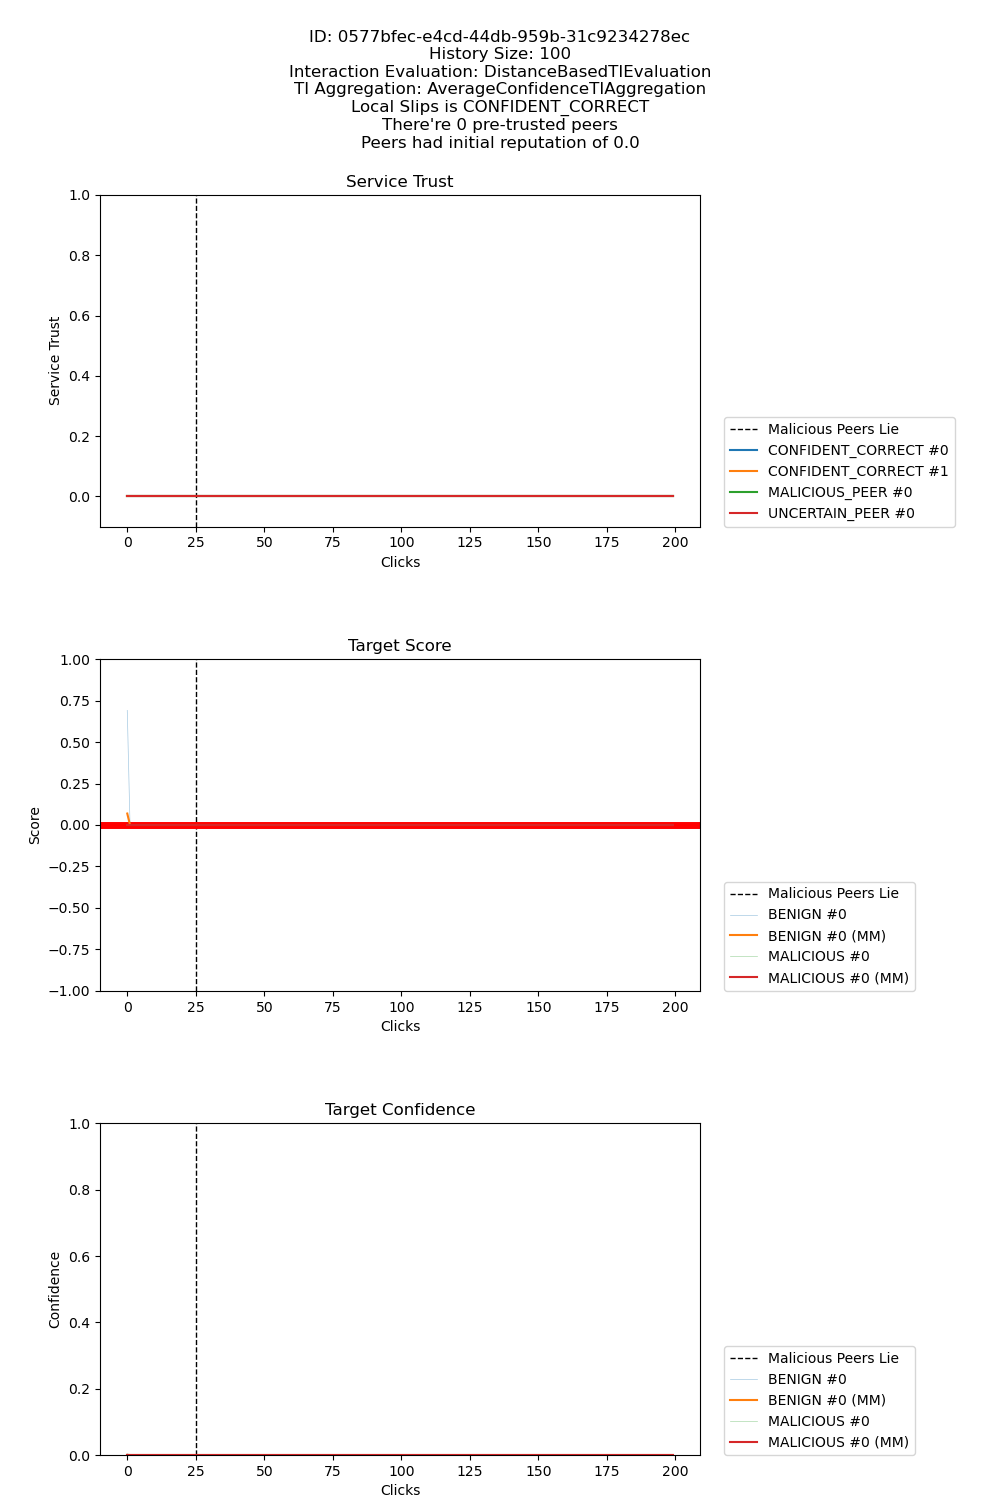
\includegraphics[width=1.0\textwidth]{assets/zero_gained_trust_all.png}
    \caption{Complete graph with all metrics from \ref{fig:zero-gained-trust}}
    \label{fig:zero-gained-trust-all}
\end{figure}

\newpage
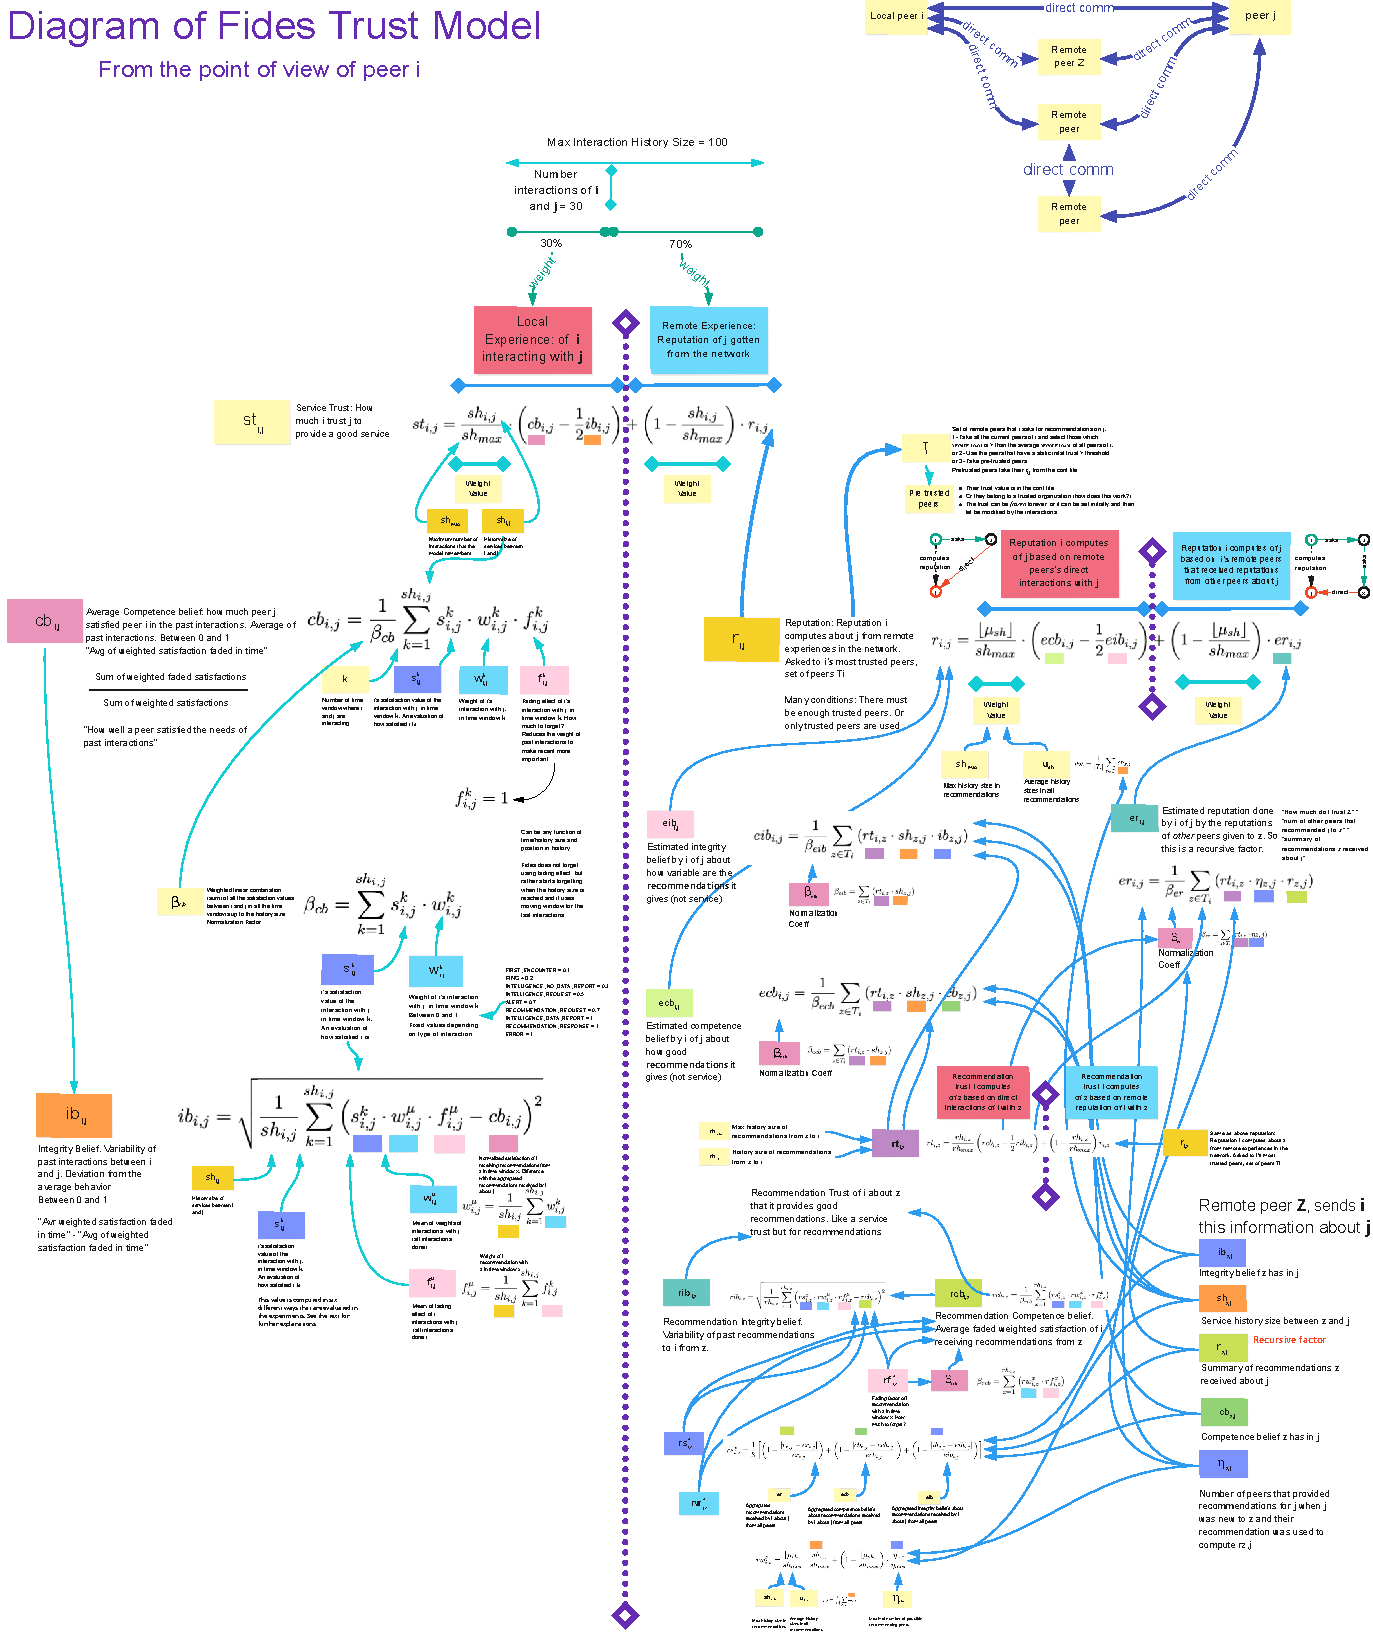
\includepdf[pages=-,scale=0.8]{assets/trust_model_scheme.pdf}